% This section of the dissertation may vary significantly in both structure and content, depending on the type of project you are undertaking. 

% The precise structure should be discussed with your supervisor, but some suggestions for additional sections are given below. The key thing to note here is that irrespective of the project type, you should \textit{justify} the choices you've made, rather than simply choosing based on expediency or familiarity. The main types of projects a student will do on the CMP9140 Research project module are below:

% · Software Development Projects

% · Research-focused projects not involving human participants

% · Research Projects involving human participants

% Its possible for a single project to adopt aspects of one or more of the types of project listed above.

% \section{Software Development Projects}

% If the primary deliverable of your project is a software product, then you should consider subsections detailing your approaches to the following:
% \begin{itemize}
%     \item Toolsets and machine environments (i.e., the software and hardware used)
%     \item Design (e.g., UML diagrams, database schema, prototypes)
%     \item Testing (i.e., the types of testing used)
% \end{itemize}
% This list is not exhaustive. For example, a games design project may include a game design document. However, it must be noted that if your project contains significant software development work, then most if not all of these sections should be present.

%This is dependent on your project’s aims/objectives and an area you must discuss with your supervisor. For example, Masters projects can encompass a range of outputs such as a significant software artefact, analysis of a dataset, development of an ML model, or development of a set of design guidelines based on a user study. It may also include a combination of different types of outputs such as a user study with app development. It is important you identify the main outputs of your project with the guidance of your supervisor and document it under this section. Any source code developed must be uploaded to the supporting documentation upload area on Blackboard


% ~2.5k words virtual coach

\section{System Requirements}
    % outline the hardware and software requirements to develop and run the system. Include specifications for computers, servers, operating systems, libraries, and frameworks.
    \subsection{Software Requirements}
        This project is designed to function on all major operating systems. The bulk of the project was programmed in a Ubuntu 22.04 environment but it has been tested on an Apple macbook and a windows laptop. To run the python scripts, there are a few libraries that are required:
        \begin{itemize}
            \item mediapipe
            \item openCV
            \item numpy
            \item pillow
            \item tkinter (normally included in python by default but not on macOS)
            \item psycopg2
        \end{itemize}
        The user data is stored locally using postgresql for the database management. This requires postgresql to be installed on the machine.
    \subsection{Hardware Requirements}
        The goal of this project was to lay the foundation for a software program that could run on a smartphone or other portable device, hence the software has relatively low hardware requirements. A camera that can parse a video signal is essential. The machines used to develop the program are:
        \begin{itemize}
            \item A Linux PC with an RTX 4070 GPU and i5-13400k CPU
            \item A Windows laptop with a GTX 1070 GPU and i7... CPU
            \item A Macbook Air M1 2020
        \end{itemize}
        Even though these machines are fairly powerful, I expect the program to be able to run on far less powerful systems.
    
\section{App Creation}
    The apps where created using Google's Mediapipe framework. Several criteria: the application must be able to detect the user's pose, the application must show the user the relevant joints and connections to the exercise, the application must be able to calculate the relevant angles within the user's pose, the application must be able to count the number of repetitions of the exercise the user has made, and the application must be able to be integrated into a python created GUI. \\

    \begin{figure}[htbp]
            \centering
            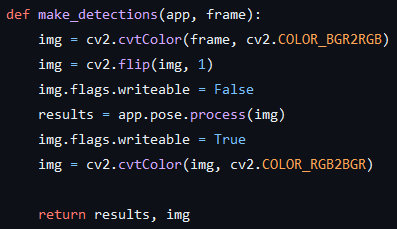
\includegraphics[width=0.49\textwidth]{figures/make_detections.png}
            \caption{Code Snippet of the make\_detections method in src/workouts/utils.py.}
            \label{fig:make_detections}
    \end{figure}
    
    The implementation of mediapipe detections can be seen in Figure \ref{fig:make_detections}. This snippet shows the raw camera input being preprocessed for the mediapipe pose processing, first the colour format is converted from BGR (openCV format) to RGB (mediapipe format), then flipped horizontally, and finally the frame's flags are set to be immutable. Once the processing of the frame is done, the flags are set to be once again mutable and the colour format is returned to BGR.

    The angle of the relevant joints to the exercise are calculated using the function seen in Figure \ref{fig:calculate_angle}. This function takes in three 2D points a, b, and c; and returns the angle between ab and cb in degrees.

    \begin{figure}[htbp]
            \centering
            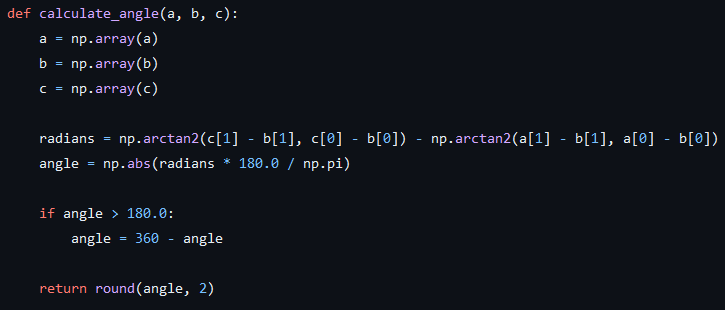
\includegraphics[width=1.00\textwidth]{figures/calculate_angle.png}
            \caption{Code Snippet of the calculate\_angle method in src/workouts/utils.py.}
            \label{fig:calculate_angle}
    \end{figure}

    Next is the repetition counting functionality which is shown in Figure \ref{fig:rep_counter}. This function is made to be generalise for it to be usable for every exercise type. It takes in as parameters the application that is using it, the current angle at the joint, the side (left or right), the low threshold the angle needs to reach for the repetition to count, the high threshold the angle needs to reach for the repetition to count, and the stage at which the muscle is at tension (or the stage that is harder to reach due to the mass of the weight). First it recovers the current count and the current rep stage, then it detects whether there has been a change in the rep stage. The rep stage will have changed from up to down if the current stage is up and the angle is above the high threshold and it will have changed from down to up if the current stage is down and the angle is below the low threshold. Then is updates the counter for the correct side.

    \begin{figure}[htbp]
            \centering
            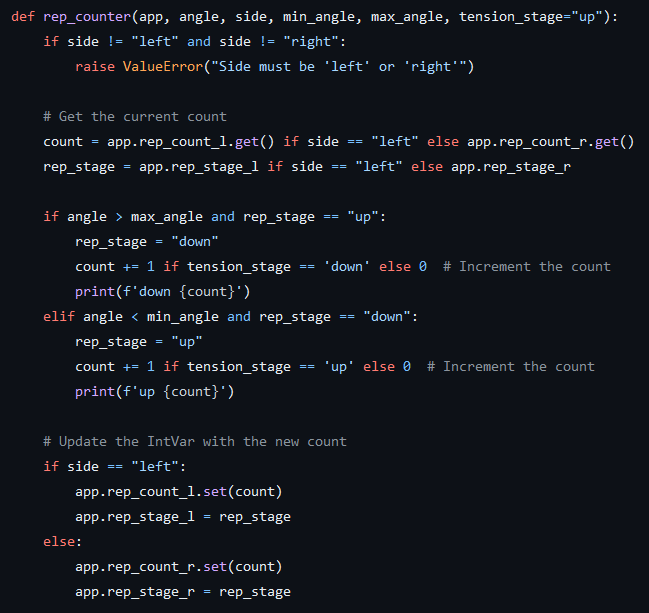
\includegraphics[width=0.75\textwidth]{figures/rep_counter.png}
            \caption{Code Snippet of the rep\_counter method in src/workouts/utils.py}
            \label{fig:rep_counter}
    \end{figure}
    
    Finally the culmination of these feature can be seen in Figure \ref{fig:detections}
    
    \begin{figure}[htbp]
            \centering
            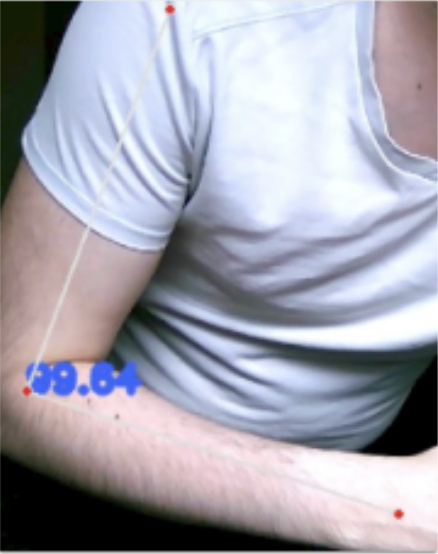
\includegraphics[width=0.34\textwidth]{figures/Screenshot 2024-08-18 at 19.07.46.png}
            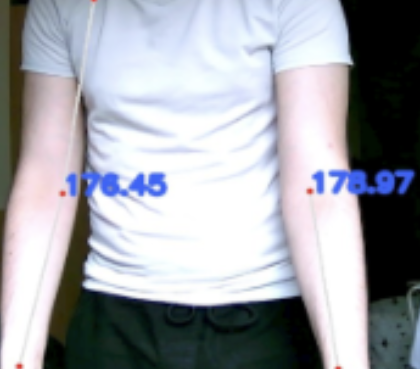
\includegraphics[width=0.49\textwidth]{figures/Screenshot 2024-08-18 at 19.08.36.png}
            \caption{Screenshots from the development of the bicep curl app. It shows mediapipe's keypoint detections on the arms and displays the angle between the shoulder-elbow segment and the wrist-elbow segment.}
            \label{fig:detections}
    \end{figure}
        
\section{GUI Creation}
    \subsection{Frontend Development}
        The frontend was developed using the tkinter library that is prepackaged into python. The GUI is organised like a tree system where each page is a node within the tree. To get to a page you must travel the GUI tree from the root node (home page) through the branches that lead to the desired page. Each branch can be traversed in both directions and the program can be exited a any moment.\\
        Here is a list of some of the pages:
        \begin{itemize}
            \item \textbf{home.py}\label{item:home}: the root node containing links to register, login, and login as guest. A screen capture of the home page can be seen below in Figure \ref{fig:home}
            \begin{figure}[htbp]
                    \centering
                    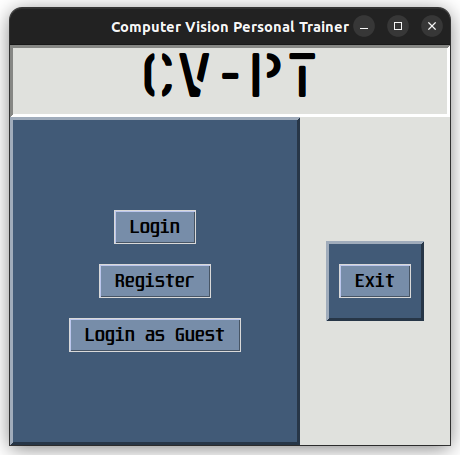
\includegraphics[width=0.49\textwidth]{figures/home.png}
                    \caption{Screen capture of the home page. (\ref{item:home})}
                    \label{fig:home}
            \end{figure}
            \item \textbf{register.py}\label{item:register}: contains a registration form that will save the users username and password to the database. If successful, it will send the user to menu.py.
            \item \textbf{login.py}\label{item:login}: contains a login form that checks if the username exists and the (hashed) password matches. If successful, it will send the user to menu.py. Screen captures of the login and register pages can be seen below in Figure \ref{fig:login_register}
            \begin{figure}[htbp]
                    \centering
                    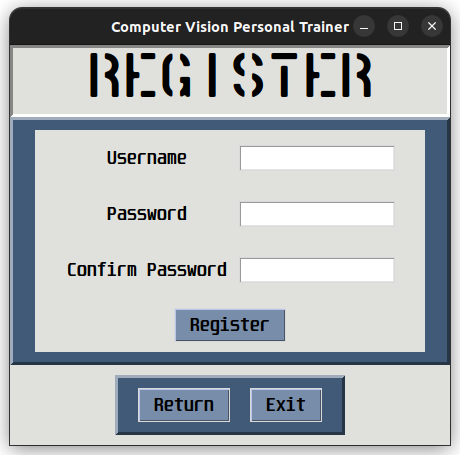
\includegraphics[width=0.49\textwidth]{figures/register.png}
                    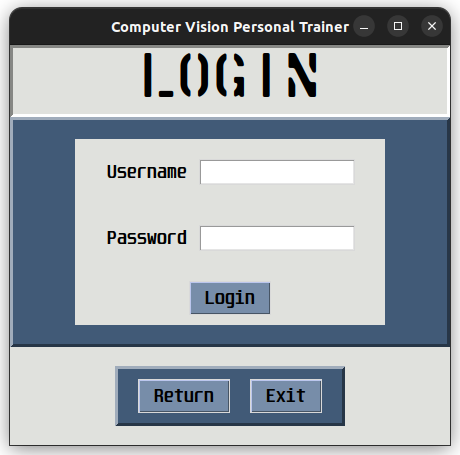
\includegraphics[width=0.49\textwidth]{figures/login.png}
                    \caption{Screen captures of the register (left \ref{item:register}) and login (right \ref{item:login}) pages.}
                    \label{fig:login_register}
            \end{figure}
            \item \textbf{menu.py}\label{item:menu}: contains a grid of buttons that link to each general muscle group/exercise type (arms, back, cardio, chest, legs, shoulders). If the user is logged in, there is also a button that links to the user's workout history. Screen captures of the menu pages with and without the history button can be seen below in Figure \ref{fig:menu}
            \begin{figure}[htbp]
                    \centering
                    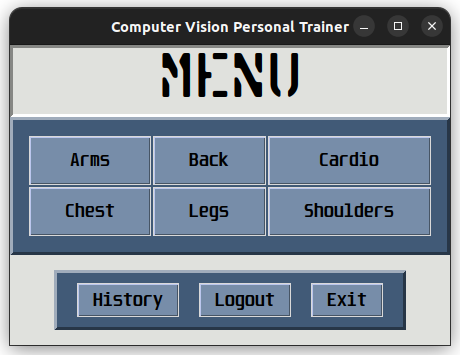
\includegraphics[width=0.49\textwidth]{figures/menu_with_login.png}
                    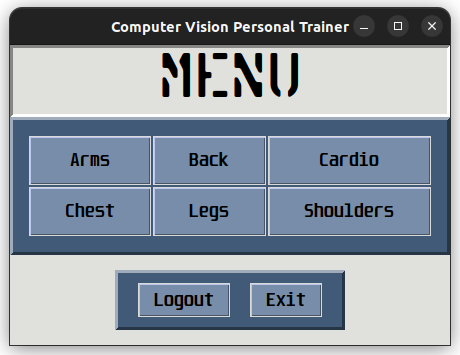
\includegraphics[width=0.49\textwidth]{figures/menu_without_login.png}
                    \caption{Screen captures of the menu page with (right) and without (left) a user logged in. (\ref{item:menu})}
                    \label{fig:menu}
            \end{figure}
            \item \textbf{arms.py}\label{item:arms}: contains a list of buttons linking to specific exercises (bicep curls and tricep pushdowns). The other child nodes of menu.py are the same where they are a list of the exercises relevant to that muscle group. A screen capture of the arms page can be seen below in Figure \ref{fig:arms}
            \begin{figure}[htbp]
                    \centering
                    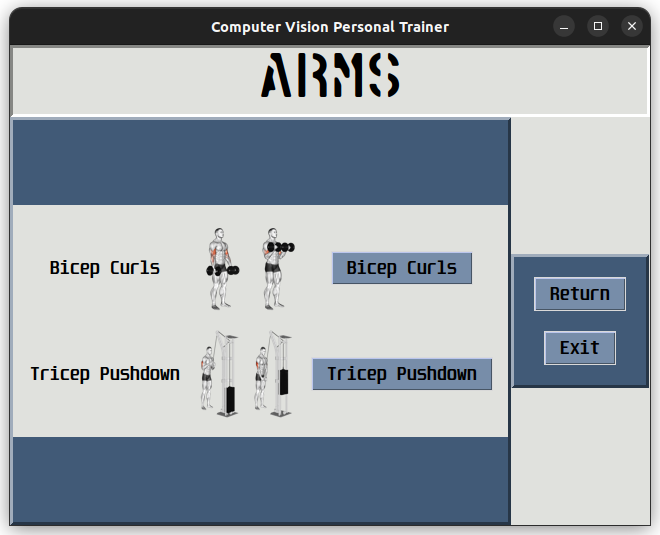
\includegraphics[width=0.49\textwidth]{figures/arms.png}
                    \caption{Screen capture of the arms page. (\ref{item:arms})}
                    \label{fig:arms}
            \end{figure}
            
            \item \textbf{bicep\_curls.py}\label{item:bicep}: These exercise pages are arranged to have a camera feed on the left half of the window and parameters and information on the right half. The camera feed will show the user what they are doing and act like the mirror in the gym, useful for visualising their form. Aswell as displaying the mediapipe skeleton on top of the joints that are relevant to the specific exercise. The right half has input areas where the user can enter the weight they are using, the amount of rest time they wish to have between sets, and depending on the exercise, which side of the body they are currently training. There is also a textbox that will display information at the top centre of the right half. A screen capture of the bicep curls app can be seen below in Figure \ref{fig:bicep}
            \begin{figure}[htbp]
                    \centering
                    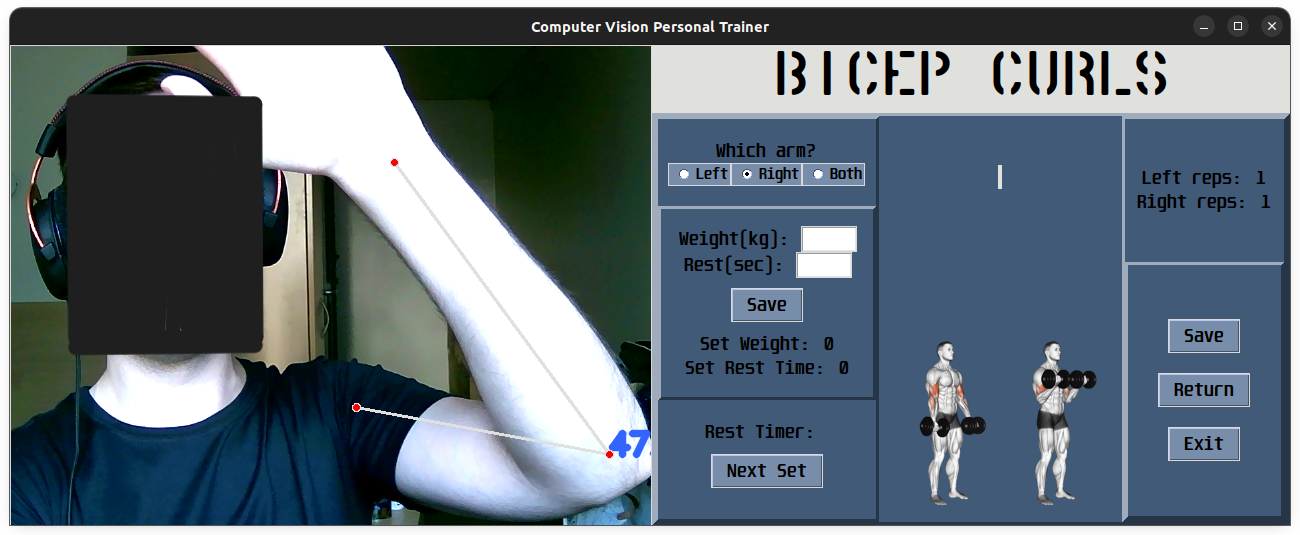
\includegraphics[width=0.99\textwidth]{figures/biceps.png}
                    \caption{Screen capture of the bicep curls page. (\ref{item:bicep})}
                    \label{fig:bicep}
            \end{figure}
        \end{itemize}

    Every time a user logs in or out, a popup appears asking them to rate their current mood on a scale of 1 to 10. This popup can be seen in Figure \ref{fig:mood}
    \begin{figure}[htbp]
            \centering
            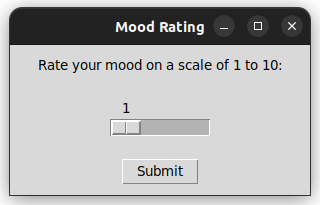
\includegraphics[width=0.49\textwidth]{figures/mood.png}
            \caption{Screen capture of the mood query popup. (\ref{item:bicep})}
            \label{fig:mood}
    \end{figure}
    
    \subsection{Backend Development}
        For the implementation of the backend I used the database management system called PostgreSQL. PostgreSQL is a relational database system written in the C programming initially released in 1996 that is free and open source. It functions also on Windows, MacOS, and Linux. As python language is also written in C, it has a strong library for database manipulation called pyscopg2.\\
        \subsubsection{Database tables}
            The schema contains three tables:
            \begin{enumerate}
                \item \textbf{users}:  (see Figure \ref{fig:users}) the users table contains five columns: 
                    \begin{itemize}
                        \item id (uuid, unique, primary key, not-null): unique identifier.
                        \item username (varchar, unique, not-null): unique username.
                        \item password (varchar, not-null): hashed password.
                        \item height (int): height of the user in centimeters, optional.
                        \item weight (int): weight of the user in kilograms, optional.
                    \end{itemize}
                    Each row refers to an individual user.
                    \begin{figure}[htbp]
                            \centering
                            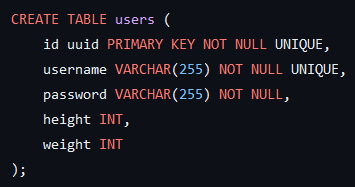
\includegraphics[width=0.67\textwidth]{figures/users.png}
                            \caption{Code Snippet of the SQL to create the users table}
                            \label{fig:users}
                    \end{figure}
                
                \item \textbf{sessions}:  (see Figure \ref{fig:sessions})the sessions table contains seven columns:
                    \begin{itemize}
                        \item id (uuid, unique, primary key, not-null): unique identifier.
                        \item username (varchar, foreign key, not-null): references the username of the user in the session.
                        \item created\_at (timestamp, not-null): timestamp at which the session started.
                        \item duration (interval): time interval between created\_at and the end of the session. Can be null because the row is created before the end of the session.
                        \item volume (int): the total weight moved by the user during the session.
                        \item start\_mood (int): the mood of the user at the start of the session on a scale of 1 to 10.
                        \item end\_mood (int): the mood of the user at the end of the session on a scale of 1 to 10.
                    \end{itemize}
                    Each row refers to an individual session.
                    \begin{figure}[htbp]
                            \centering
                            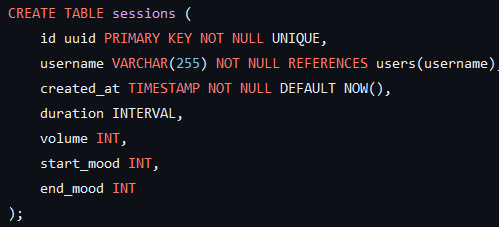
\includegraphics[width=0.67\textwidth]{figures/sessions.png}
                            \caption{Code Snippet of the SQL to create the users table}
                            \label{fig:sessions}
                    \end{figure}
                
                \item \textbf{workouts}:  (see Figure \ref{fig:workouts}) the workouts table contains eight columns:
                    \begin{itemize}
                        \item id (uuid, unique, primary key, not-null): unique identifier.
                        \item session\_id (uuid, foreign key, not-null): references the id of the session the workout belongs to.
                        \item name (varchar, not-null): the name of the excerce being performed by the user (e.g. bicep curls)
                        \item created\_at (timestamp, not-null): timestamp at which the workout started.
                        \item duration (interval): time interval between created\_at and the end of the workout. Can be null because the row is created before the end of the workout.
                        \item reps (int): number of repetitions the user performed during the workout.
                        \item max\_weight (int): the weight in kilograms lifted during the heaviest set during the workout.
                        \item volume (int): the sum of the number of reps times the weight of the set for each set performed during the workout.
                    \end{itemize}
                    Each row refers to an individual workout.
                    \begin{figure}[htbp]
                            \centering
                            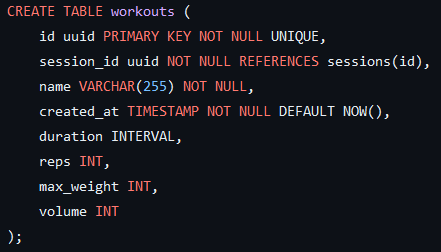
\includegraphics[width=0.67\textwidth]{figures/workouts.png}
                            \caption{Code Snippet of the SQL to create the workouts table}
                            \label{fig:users}
                    \end{figure}
                
            \end{enumerate}
            Another functionality that is provided by postgresql is the ability to create functions, also known as routines, to preform multiple SQL queries and actions.\\

        \subsubsection{Register functionality}
            The register system (see Figure \ref{fig:register} functions as follows: first there is a equality check between the password and the confirm password entries inputted by the user. If they match, then a connection to the database is made with DBConnection (see Figure \ref{fig:DBConnection}). 

            \begin{figure}[htbp]
                    \centering
                    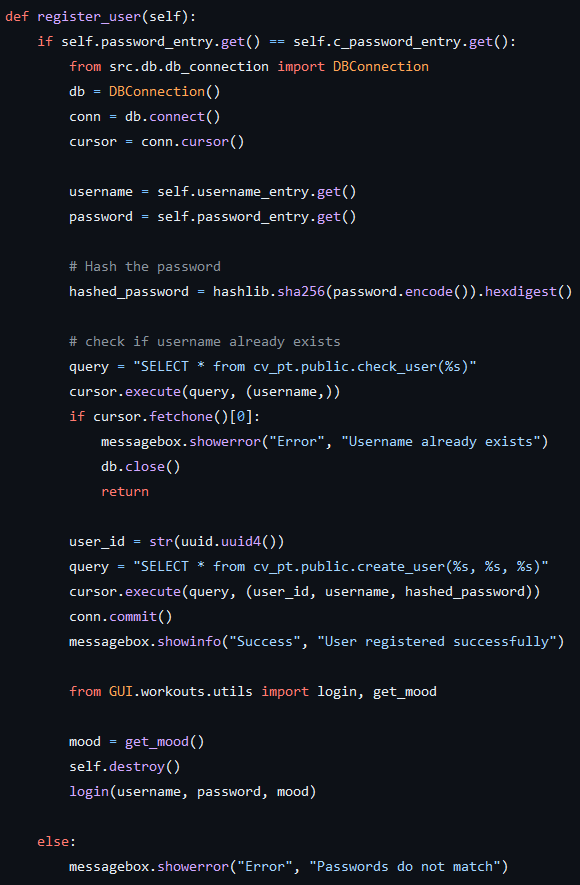
\includegraphics[width=0.9\textwidth]{figures/register_code.png}
                    \caption{Code Snippet of the register function}
                    \label{fig:register}
            \end{figure}

            Then, the password is hashed using the sha256 hashing function, and the users table is scanned for the username. If the username already exists, the process is stopped and the user is notified though a messagebox that their chosen username is already taken. Else, if the username is not taken, a new user is added to the users table with a universally unique identifier (uuid), the username, and the hashed password. The user is then automatically logged in (the login process is described next). 

        \subsubsection{Login functionality}
            The login system (see Figure \ref{fig:login_code}) functions as follows: first a connection to the database is formed using DBConnection (see Figure \ref{fig:DBConnection}).
            
            \begin{figure}[htbp]
                    \centering
                    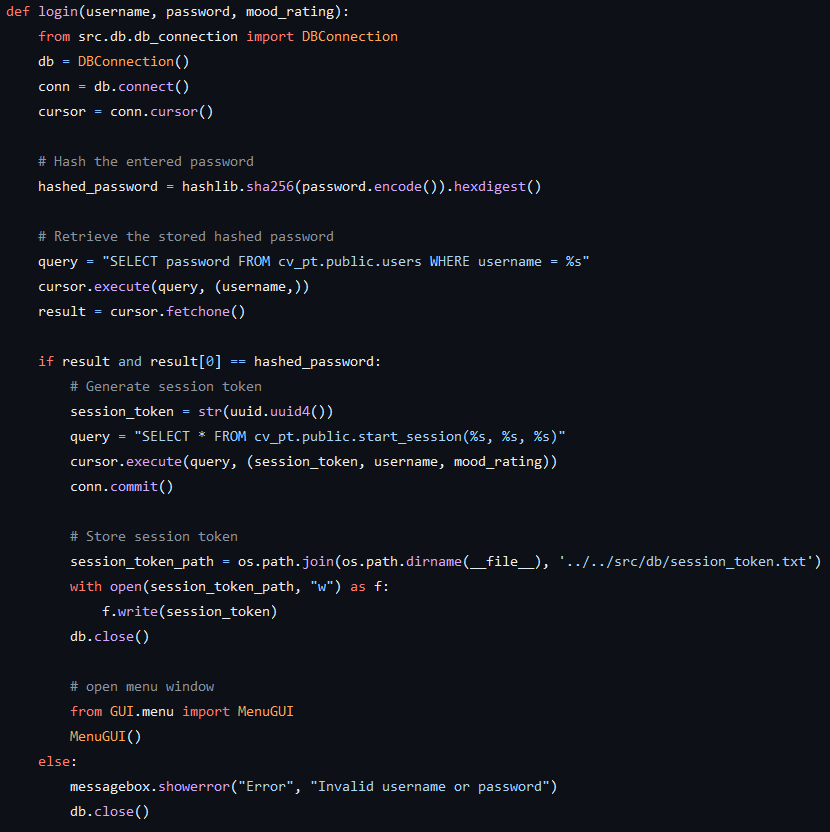
\includegraphics[width=0.99\textwidth]{figures/login_code.png}
                    \caption{Code Snippet of the login function}
                    \label{fig:login_code}
            \end{figure}

            Following that, the password entered by the user is hashed using the same hashing algorithm used for the encryption of the passwords and the database is searched for a user who has both matching username and hashed password. If a user is found, a new session is created, with a uuid which acts as the session token. This token is both stored in the database and also a newly created text file that only exists if a user is logged in.

            \begin{figure}[htbp]
                    \centering
                    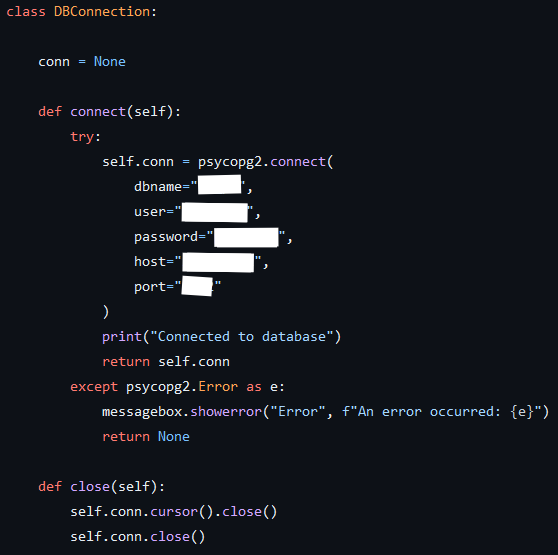
\includegraphics[width=0.67\textwidth]{figures/DBConnection.png}
                    \caption{Code Snippet of the DBConnection Class}
                    \label{fig:DBConnection}
            \end{figure}
            
            Finally, the menu GUI page is opened. If there are no matching users, a messagebox appears notifying the user that either the username or password is invalid and the connection to the database is closed. Which one of the username and password being invalid is not specified for security reasons, because if there is an indication that the username exists, it would be easier to brute force a login.\\  

            Figure \ref{fig:DBConnection} shows how to connect to a postgresql database using the psycopg2 library in python. 
        
    \section{Testing and Debugging}
    % Discuss the methods and tools used to test the system for functionality, performance, and reliability. Include the process of identifying and fixing bugs or issues.
    \subsection{Integration Testing}
        Testing whether the integration of the application into the GUI was fairly simple. All that needed to be done was to run the program and see if it displays. The first issue encountered was how to convert the default popup window openCV produces into a tkinter frame. This was solved by having the application be initialised as a tkinter frame by wrapping it in a class that inherits from ttk.Frame and running $super().\_\_init\_\_(parent)$ where $parent$ is a parameter of the application.\\
        The second issue was that the application would not open if an application had previously been opened during the program's uptime. This was caused by the application not closing properly when the window was closed. This was solved by creating a close method in the application class that destroys the application (see Figure \ref{fig:close}) and calling it when closing the window.
        
        \begin{figure}[htbp]
                \centering
                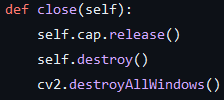
\includegraphics[width=0.49\textwidth]{figures/close.png}
                \caption{Code Snippet of the close method in src/workouts/arms/bicep\_curls.py}
                \label{fig:close}
        \end{figure}

    \subsection{System Testing}
        For the testing of the backend system, no major bugs where encountered as I have had previous experience with setting up a postgresql database in the past and had knowledge on how to avoid issues. I must also say that the integration of database management in PyCharm facilitated the task significatly.